\section{Appendix: Kinestatic Filtering}

\begin{frame}{How to write $\vec{a}_{cmd}$ using a selection matrix $S$}
  A selection matrix $S$ \alert{may} be used to separate the force-controlled 
  and position-controlled \emph{reciprocal} subspaces
  \begin{columns}
    \begin{column}{0.6\textwidth}
      \[  
      \prescript{ws}{}{\vec{a}}_{cmd} = S 
        \begin{bmatrix}
          a_{cmd,x} \\
          a_{cmd,y} \\
          * \\
          \vec{a}_{cmd,\Phi}
        \end{bmatrix} + (I - S) 
        \begin{bmatrix}        
          * \\ * \\ a_{cmd,z} \\ * \\ * \\ *
        \end{bmatrix}
      \]
    \end{column}
    \begin{column}{0.35\columnwidth}
      \[
      S =
        \begin {bmatrix}
          1 & 0 & 0 & 0 & 0 & 0\\
          0 & 1 & 0 & 0 & 0 & 0\\
          0 & 0 & 0 & 0 & 0 & 0\\
          0 & 0 & 0 & 1 & 0 & 0\\
          0 & 0 & 0 & 0 & 1 & 0\\
          0 & 0 & 0 & 0 & 0 & 1\\
        \end {bmatrix}
      \]
    \end{column}
  \end{columns}
\end{frame}

\begin{frame}{A different interpretation of the selection matrix}
  Position controlled and force controlled subspaces can be seen in terms of
  \emph{natural} and \emph{artificial} constraints:
  \begin{itemize}
  \item[-]natural: directions along which the end effector can not move and exert forces
  \item[-]artificial: directions along which the end effector can move and exert forces
  \end{itemize}
  \par
  Artificial constraints directions belong to the span of appropriate matrices
\end{frame}

\begin{frame}{An example}
  Consider admissible twists and wrenches projected in $ws$
  \begin{columns}
    \begin{column}{0.4\columnwidth}
      \[
      B=
      \begin {bmatrix}
        1 & 0 & 0 & 0 & 0\\
        0 & 1 & 0 & 0 & 0\\
        0 & 0 & 0 & 0 & 0\\
        0 & 0 & 1 & 0 & 0\\
        0 & 0 & 0 & 1 & 0\\
        0 & 0 & 0 & 0 & 1
      \end {bmatrix}
      \]
    \end{column}
    \begin{column}{0.2\columnwidth}
      \[
      a=
      \begin {bmatrix}
        0 \\
        0 \\
        1 \\
        0 \\
        0 \\
        0 
      \end {bmatrix}
      \]
    \end{column}
    \begin{column}{0.4\columnwidth}
      \[
      \begin{split}
        & \prescript{ws}{}{\boldsymbol{\xi}}_{adm} \in \mathcal{R}(B)\\
        & \prescript{ws}{}{\vec{w}}_{adm} \in \mathcal{R}(a)
      \end{split}
      \]
    \end{column}
  \end{columns}

  The most general motion is that of a translation ($x$-$y$ direction of $ws$)
  and/or a rotation about some axis that pass through a point $P$, e.g. the center of the 
  palm of the hand.
  \par
  Force can only be exerted along the $z$ direction of $ws$. No torques are allowed.
  \end{frame}

\begin{frame}{An example (continued)}
  In order to filter out undesired twists and wrenches the following projection matrices are used (Kinestatic filter)
  \begin{columns}
    \begin{column}{0.4\columnwidth}
      \begin{flalign*}
        &P_B = B (B^T B)^{-1} B^T\\
        &P_B \vec{e}_i = \vec{e}_i \quad i \in \{1, 2, 4, 5, 6\}\\
        &P_B \vec{e}_3 = \vec{0}
      \end{flalign*}
    \end{column}
    \begin{column}{0.4\columnwidth}
      \begin{flalign*}
        &P_a = a (a^T a)^{-1} a^T&\\
        &P_a \vec{e}_i = \vec{0} \quad i \in \{1, 2, 4, 5, 6\}\\
        &P_a \vec{e}_3 = \vec{e}_3
      \end{flalign*}
    \end{column}
  \end{columns}
  \par
  The projectors lead to the already seen selection matrices $S = P_B$ and $I-S = P_a$
\end{frame}

\begin{frame}{A more general example}
  In general twists/wrenches can be commanded with respect to a
  different reference point $E'$ for example $EE' = \begin{bmatrix} \bar{x} & 0 & 0 \end{bmatrix}^T$
  \begin{columns}
    \begin{column}{0.4\columnwidth}
      \begin{flalign*}
        &{}^{ws}\boldsymbol{\xi}' = K(\bar{x}) ({}^{ws}\boldsymbol{\xi})\\
        &B' = K B =
        \left[
          \begin{smallmatrix}
            1 & 0 & 0 & 0 & 0 \\
            0 & 1 & 0 & 0 & x \\
            0 & 0 & 0 & -x & 0 \\
            0 & 0 & 1 & 0 & 0 \\
            0 & 0 & 0 & 1 & 0 \\
            0 & 0 & 0 & 0 & 1 
          \end{smallmatrix}
          \right]
      \end{flalign*}
    \end{column}
    \begin{column}{0.4\columnwidth}
      \begin{flalign*}
        &{}^{ws}\vec{w}' = G(\bar{x}) ( {}^{ws}\vec{w})\\
        &a' = G a =
        \left[
          \begin{smallmatrix}
            0 \\
            0 \\
            1 \\
            0 \\
            x \\
            0 
          \end{smallmatrix}
          \right]
      \end{flalign*}
    \end{column}
  \end{columns}
  However using the standard projector gives for example
  \begin{columns}
    \begin{column}{0.4\columnwidth}
      \begin{flalign*}
        &P_B' K \vec{e}_3 =
        \left[
          \begin{smallmatrix}
            0 & 0 & \textcolor{red}{\frac{x^2}{x^2+1}} & 0 & \textcolor{red}{-\frac{x}{x^2+1}} & 0
          \end{smallmatrix}
          \right]^T
      \end{flalign*}
    \end{column}
    \begin{column}{0.4\columnwidth}
      \begin{flalign*}
        &P_a' G \vec{e}_5 =
        \left[
          \begin{smallmatrix}
            0 & 0 & \textcolor{red}{\frac{x}{x^2+1}} & 0 & \textcolor{red}{\frac{x^2}{x^2+1}} & 0
          \end{smallmatrix}
          \right]^T
      \end{flalign*}
    \end{column}
  \end{columns}
\end{frame}

\begin{frame}{An invariant filter [Marescotti, Bonivento and Melchiorri, 1990]}
  An invariant filter behaves well even when the reference point changes
  \begin{columns}
    \begin{column}{0.5\columnwidth}
      \begin{block}{$P_B'' = K P_B K^{-1}$}
        \vskip-0.1in
        \[
        \begin{split}
          \text{If } & P_B ({}^{ws}\boldsymbol{\xi}) = {}^{ws}\boldsymbol{\xi}\\
          \text{then } &P_B'' ({}^{ws}\boldsymbol{\xi}') = P_B'' K ({}^{ws}\boldsymbol{\xi}) \\
          &=K P_B K^{-1} K ({}^{ws}\boldsymbol{\xi})\\
          &=K P_B ({}^{ws}\boldsymbol{\xi})\\
          &=K ({}^{ws}\boldsymbol{\xi}) = {}^{ws}\boldsymbol{\xi}'
        \end{split}
        \]
        \[
        \begin{split}
          \text{If } & P_B ({}^{ws}\boldsymbol{\xi}) = \vec{0}\\
          \text{then } &P_B'' ({}^{ws}\boldsymbol{\xi}') =K P_B ({}^{ws}\boldsymbol{\xi})\\
          &= \vec{0}
        \end{split}
        \]
      \end{block}
    \end{column}
    \begin{column}{0.5\columnwidth}
      \begin{block}{$P_a'' = G P_a G^{-1}$}
        \vskip-0.1in
        \[
        \begin{split}
          \text{If } & P_a ({}^{ws}\vec{w}) = {}^{ws}\vec{w}\\
          \text{then } &P_a'' ({}^{ws}\vec{w}') = P_a'' G ({}^{ws}\vec{w}) \\
          &=G P_a G^{-1} G ({}^{ws}\vec{w})\\
          &=G P_a ({}^{ws}\vec{w})\\
          &=G ({}^{ws}\vec{w}) = {}^{ws}\vec{w}'
        \end{split}
        \]
        \[
        \begin{split}
          \text{If } & P_a ({}^{ws}\vec{w}) = \vec{0}\\
          \text{then } &P_a'' ({}^{ws}\vec{w}') =G P_a ({}^{ws}\vec{w})\\
          &= \vec{0}
        \end{split}
        \]
      \end{block}
    \end{column}
  \end{columns}
\end{frame}

\begin{frame}[shrink=30]
  \frametitle{Kinestatic filtering}
  \framesubtitle{Combining HIC with the kinestatic filtering}
  Since the kinestatic filtering is applied to twists and wrenches
  it is not possible to apply it directly to the commanded accelerations
  described above.\\
  Anyway, as observed in [Marescotti, Bonivento and Melchiorri, 1990],
  there is no necessity to use the alternative projectors $P_B''$ and
  $P_a''$ in the control algorithm since twists and wrenches expressed
  with respect to another reference point can always be transformed back
  to their original form using the inverse transformations $K^{-1}$ and
  $G^{-1}$.\\
  In that case the projection matrices always reduce to the selection matrices
  $S$ and $I-S$ that are also suitable to filter undesired commanded accelerations.
  \begin{center}
    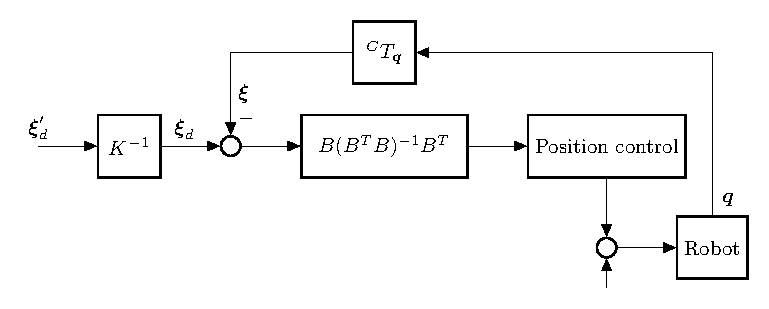
\includegraphics[scale=1]{kinestatic_filtering}
  \end{center}
\end{frame}
